\documentclass[10pt,aspectratio=169, colorlinks=true, linkcolor=circlBlue]{beamer}

% tlp allowed values: clear, green, amber, amber+strict, red
\usetheme[numbering=fraction, progressbar=frametitle, tlp=clear]{circl}

% for code highlighting
\usepackage{minted}
% to draw pingus
\usepackage{tikzpingus}
% to draw boxes to catch attention
\usepackage{awesomebox}
% For hyperlinks in the document and PDF metadata
\usepackage{hyperref}
% useful only if we want to customize minted background
\usepackage{tcolorbox}
%useful to make image side by side
\usepackage{caption}
\usepackage{subcaption}

\hypersetup{
    pdftitle={Flowintel},    % Title
    pdfauthor={David Cruciani},               % Author
    pdfsubject={Flowintel, support analysts to organise their case and tasks }, % Subject
    pdfkeywords={Flowintel, case management}, % Keywords
    colorlinks=false,                       % Color links instead of boxes
    linkcolor=blue,                        % Color of internal links
    citecolor=blue,                        % Color of citations
    urlcolor=blue                          % Color of external links
}

% set the logo to put in the title page
\titlegraphic{\noindent\hfill
\includegraphics[width=0.25\textwidth]{img/logo-circl.pdf}}
\title{Flowintel - WARFARE}
% \subtitle{2025 presentation - Luxembourg}
\date{April, 2026}

\institute{CIRCL \normalurl{https://www.circl.lu}}
% if set inserts a title link into the title page
\titlelink{\faGithub\space \normalurl{https://github.com/flowintel/flowintel}}

\begin{document}

% include custom commands
\include{commands.tex}


% Title page
\begin{frame}
	\titlepage%
\end{frame}


% \section{Origin of the project}
\begin{frame}[t]{Flowintel, What \& Why }
	\begin{figure}[H]
		\centering
		
\includegraphics[width=0.15\textwidth]{img/flowintel_logo.png}
	\end{figure}
	\textbf{FlowIntel} is an open-source incident \& forensic case management platform.
	\begin{itemize}
		\item Day-to-day CSIRT / SOC work still relies on spreadsheets, generic ticketing tools, or expensive closed platforms.
		\item There was \textbf{no vendor-neutral, open source} alternative focused on security operations workflows.
		\item FlowIntel fills that gap: structure investigations, keep evidence organised, and accelerate collaboration.
	\end{itemize}

\end{frame}

\begin{frame}{Overview - Homepage}
	\begin{figure}[H]
		\centering
		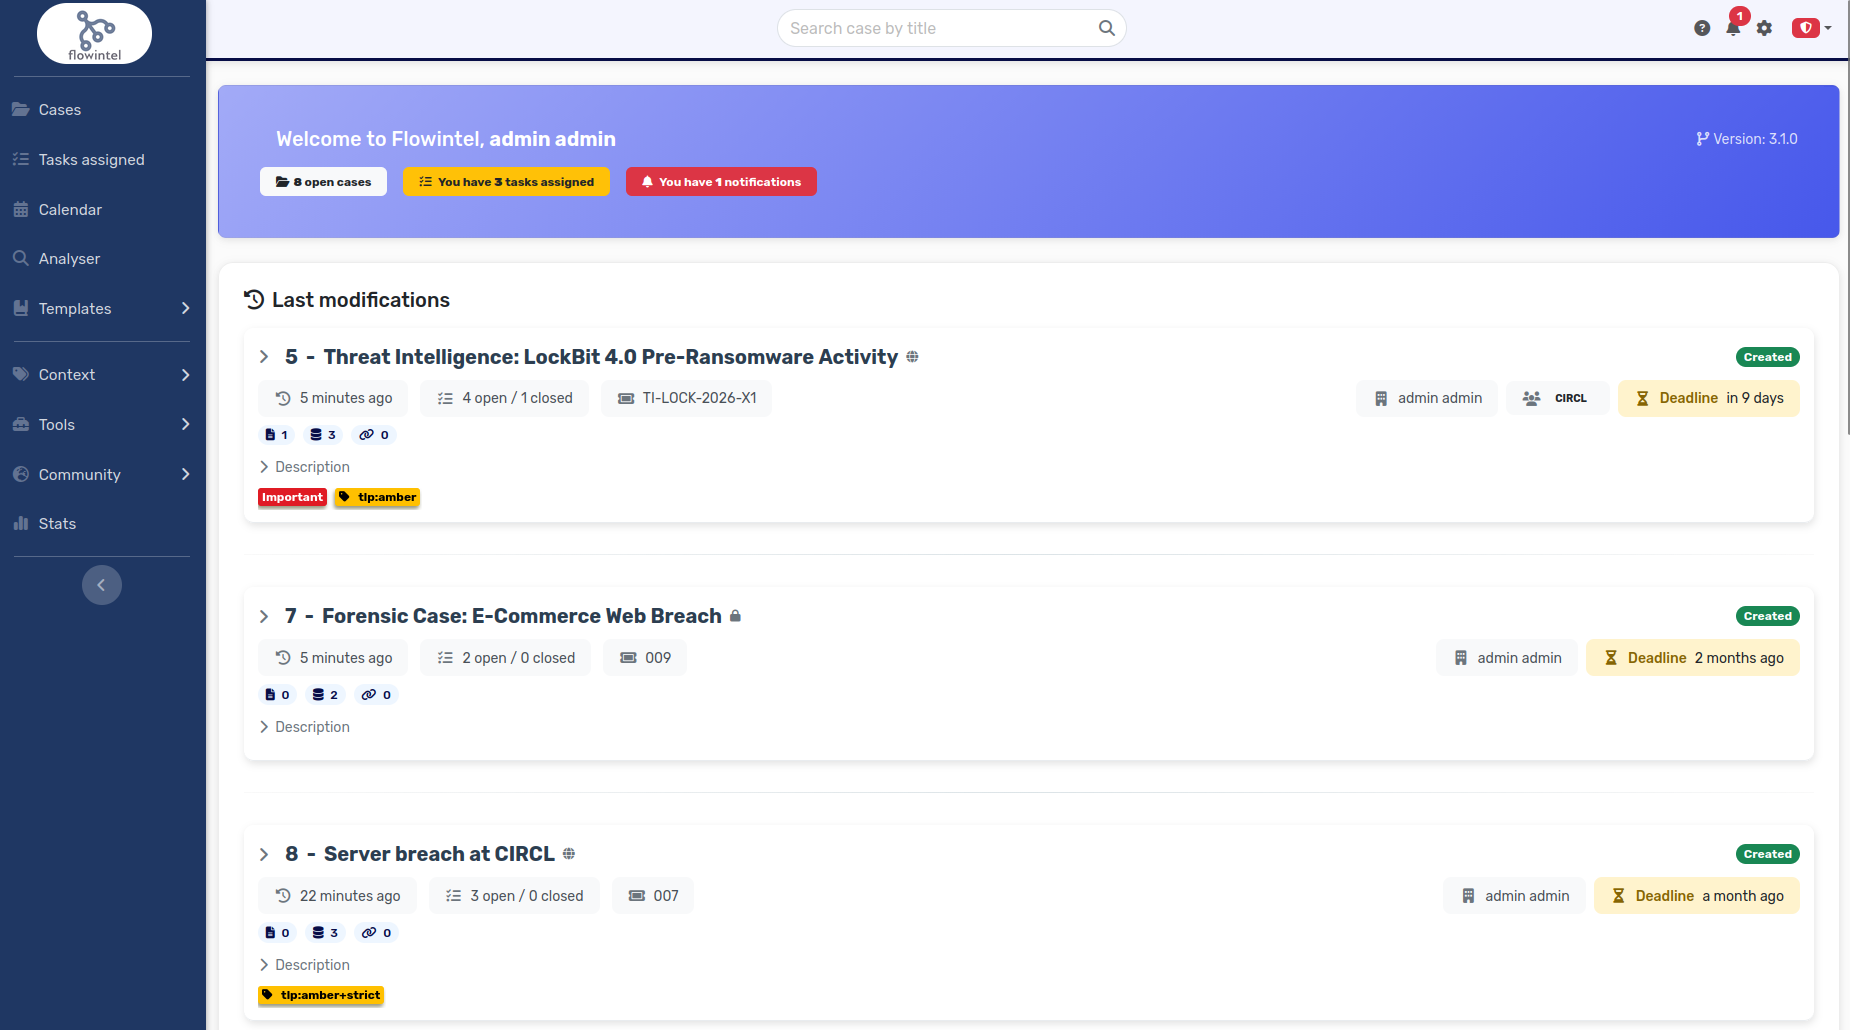
\includegraphics[width=0.9\textwidth]{img/home.png}
	\end{figure}
\end{frame}

\section{1. Manage Structured Investigations}

\begin{frame}{1. Manage Structured Investigations}
	\begin{itemize}
		\item Create and manage cases with {\bf full lifecycle tracking}
		\item Break cases into tasks and subtasks
		\item Assign {\bf investigators with role-based access}
		\item Track progress, deadlines, and workload
		\item Keep notes organized
		\item Use case and task templates for standardized procedures
	\end{itemize}
\end{frame}

\begin{frame}{1. Manage Structured Investigations - case}
	\begin{figure}[H]
		\centering
		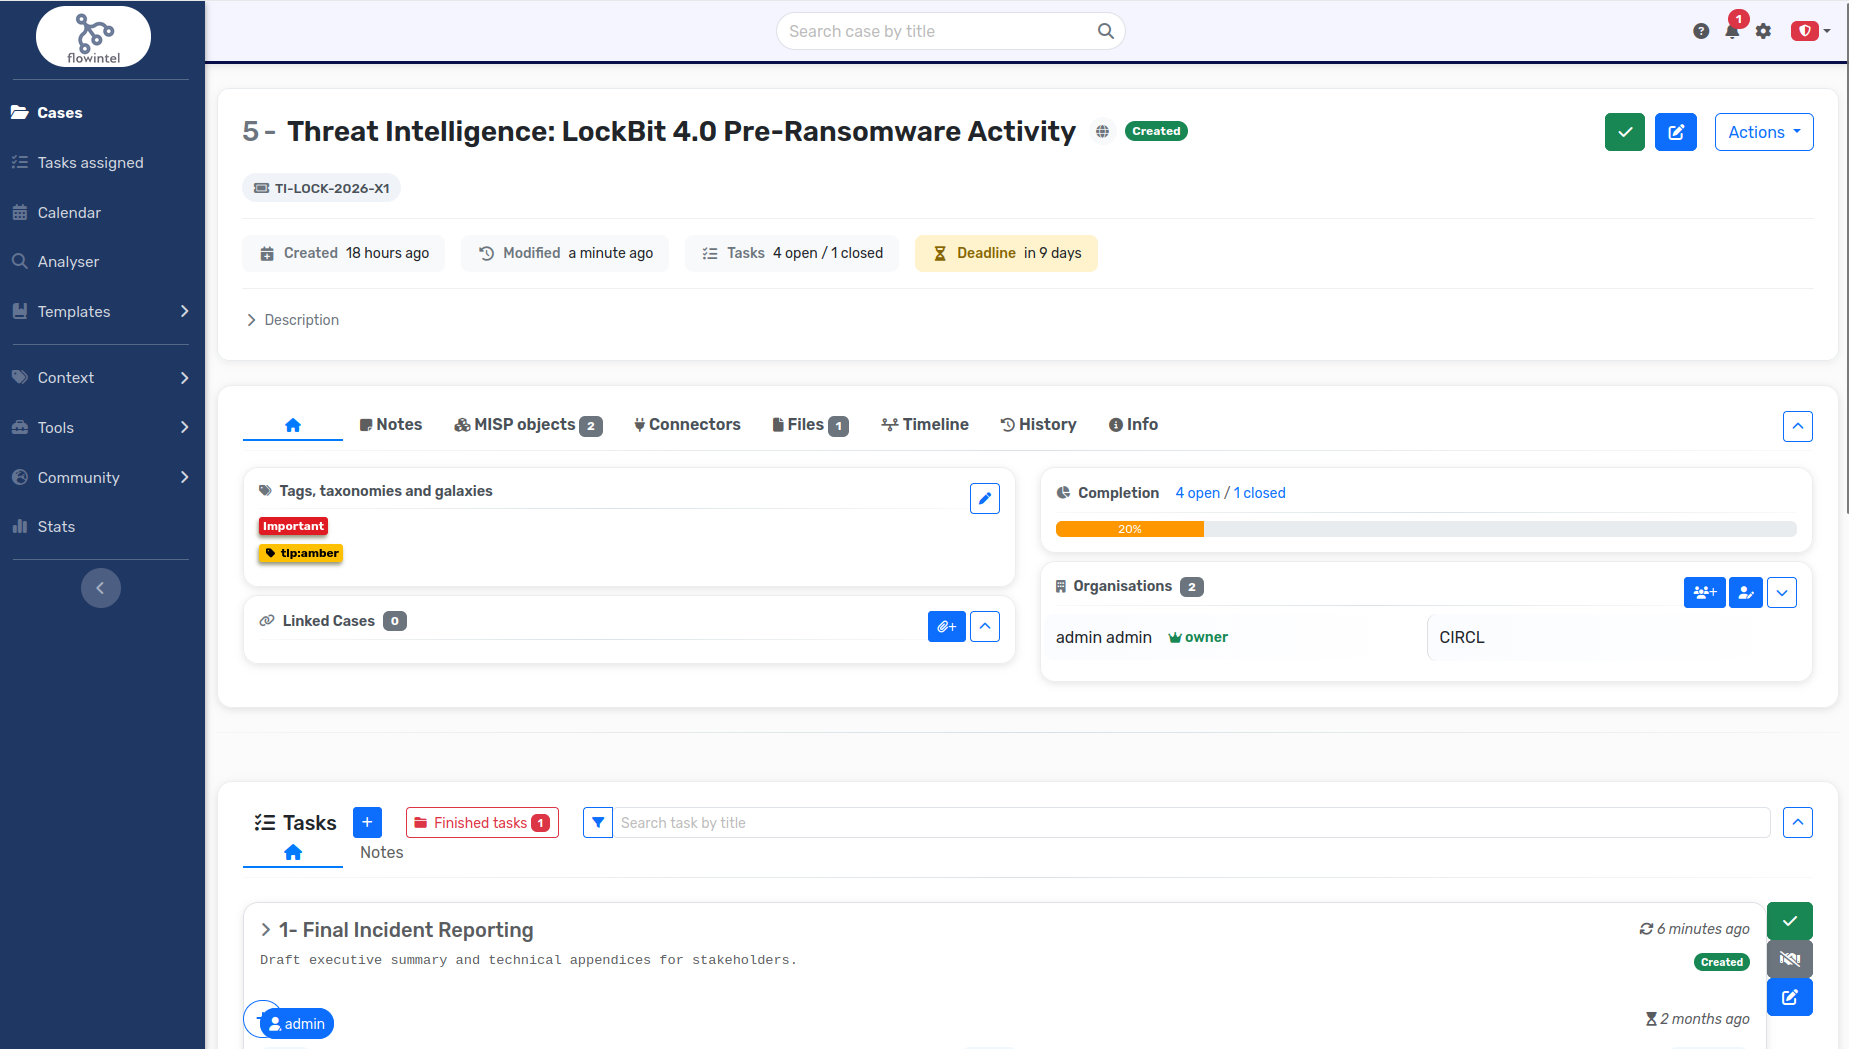
\includegraphics[width=0.9\textwidth]{img/case_view.png}
	\end{figure}
\end{frame}

\begin{frame}{1. Manage Structured Investigations - Notes}
	\begin{figure}[H]
		\centering
		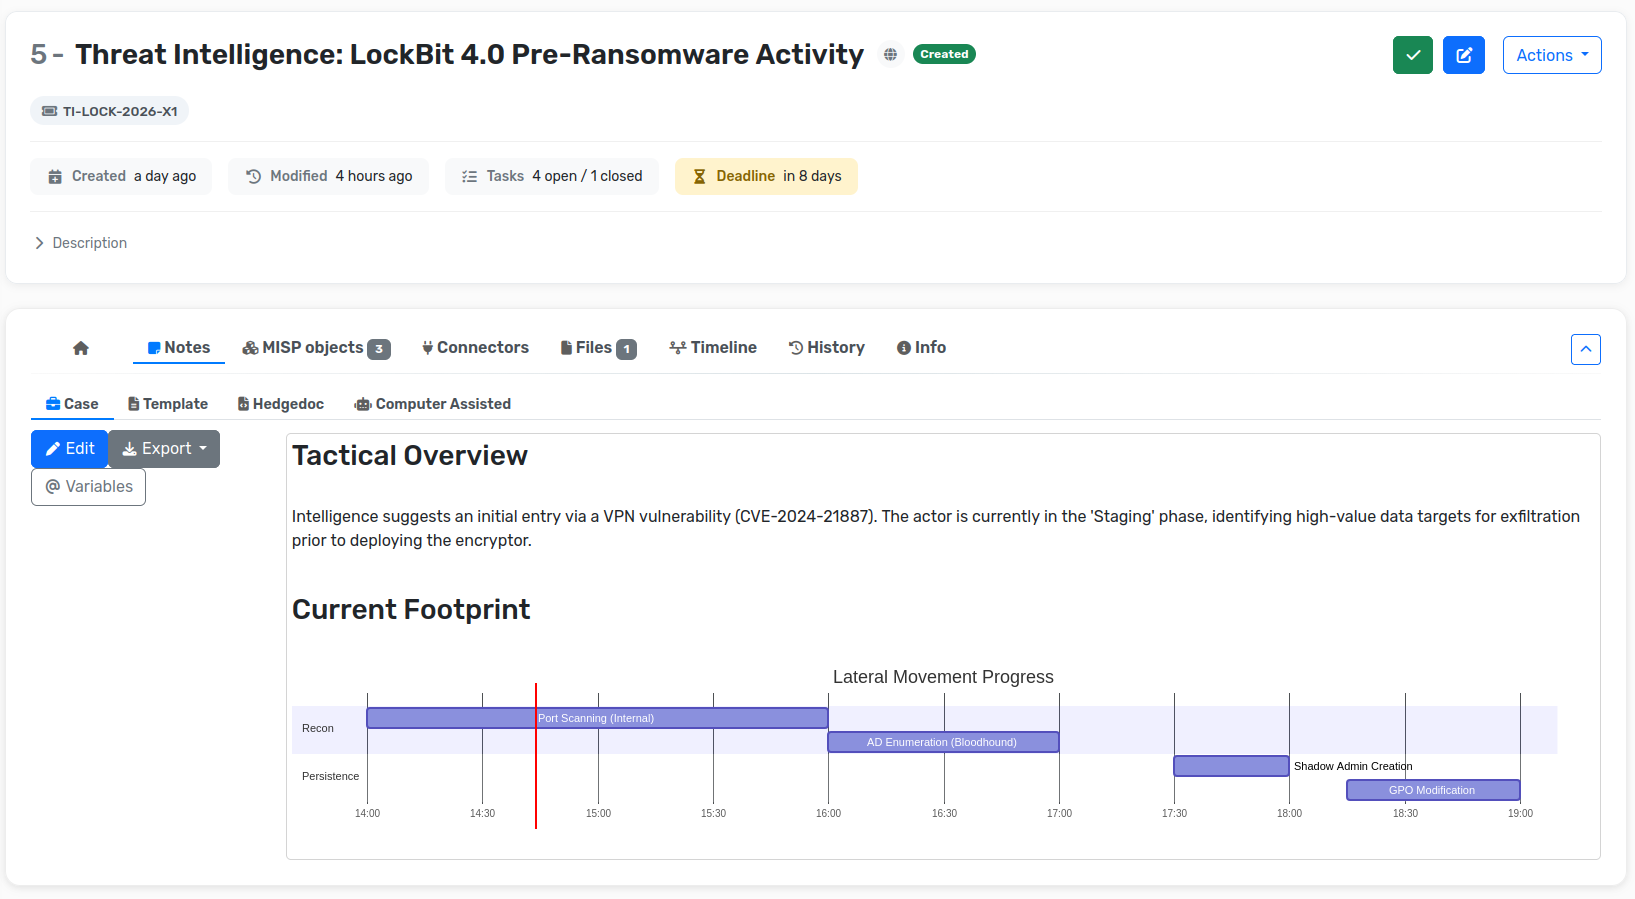
\includegraphics[width=0.9\textwidth]{img/note_view.png}
	\end{figure}
\end{frame}

\begin{frame}{1. Manage Structured Investigations - timeline}
	\begin{figure}[H]
		\centering
		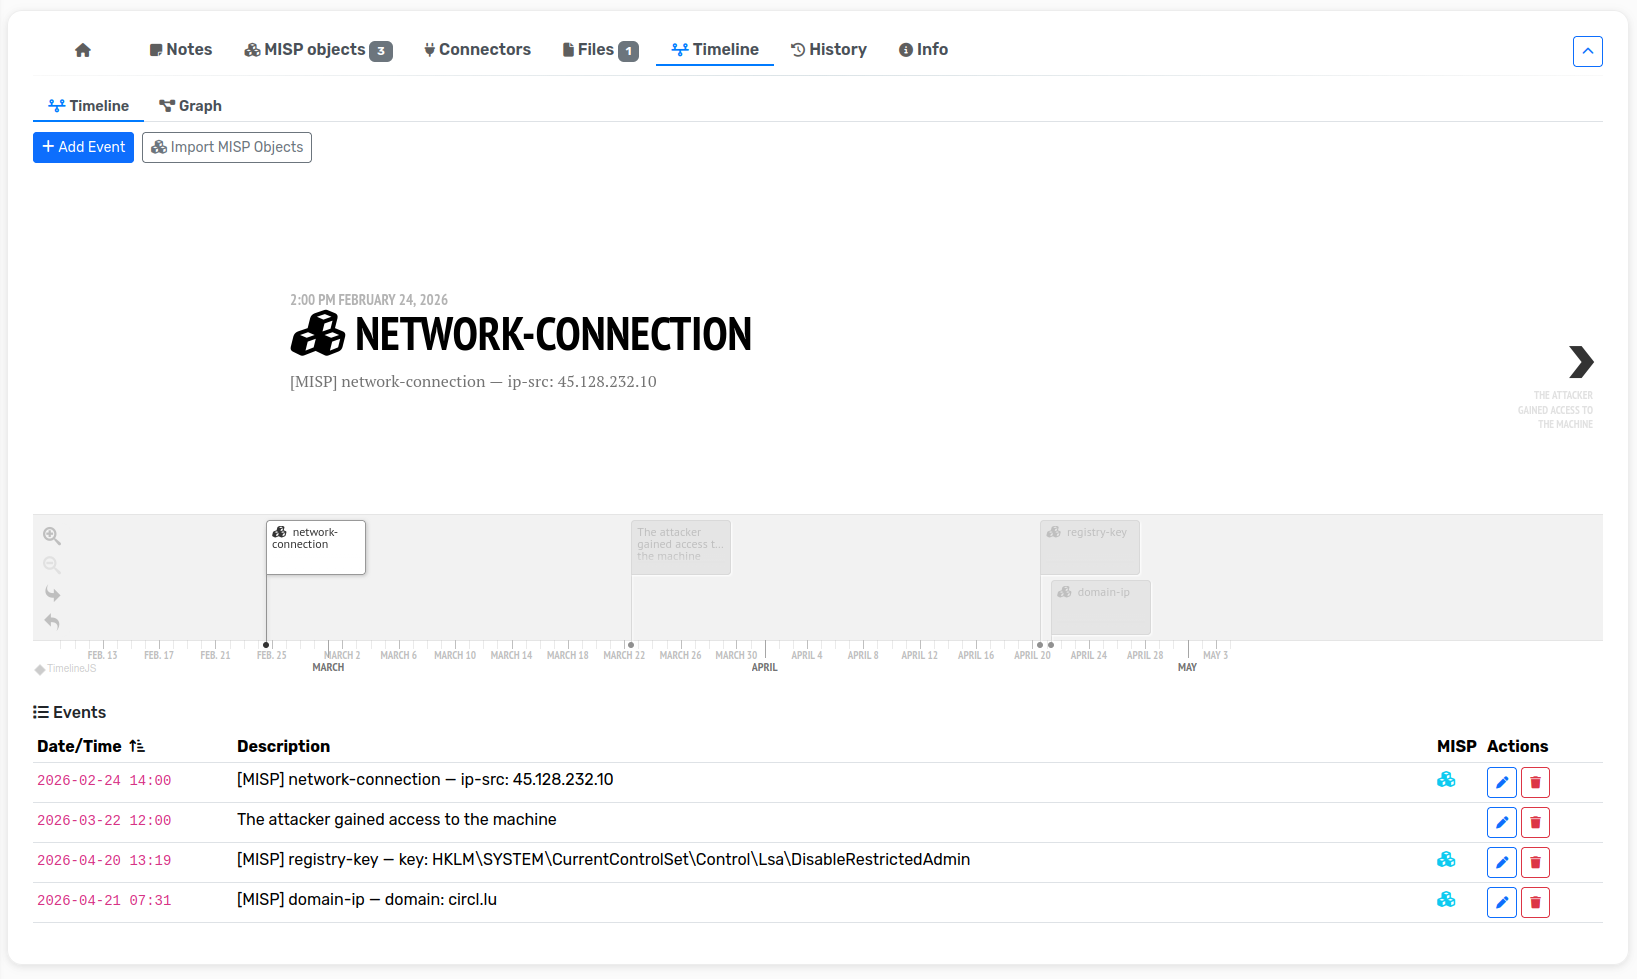
\includegraphics[width=0.9\textwidth]{img/timeline_view.png}
	\end{figure}
\end{frame}

\begin{frame}{1. Manage Structured Investigations - graph}
	\begin{figure}[H]
		\centering
		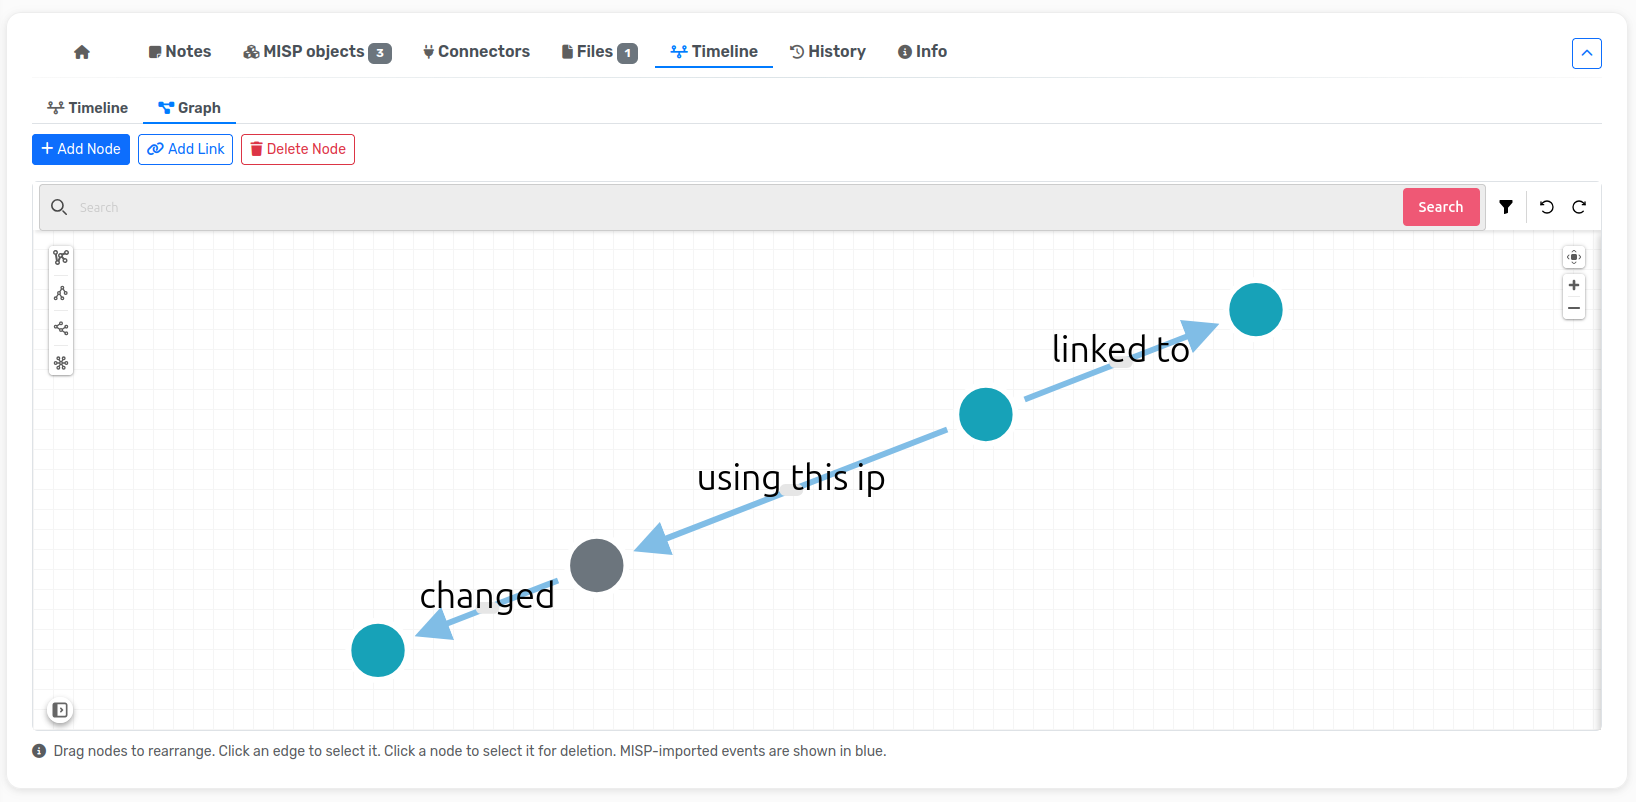
\includegraphics[width=0.9\textwidth]{img/graph_view.png}
	\end{figure}
	\textit{\small made with Pivotick: } \url{https://pivotick.github.io/Pivotick/}
\end{frame}

\begin{frame}{1. Manage Structured Investigations - task}
	\begin{figure}[H]
		\centering
		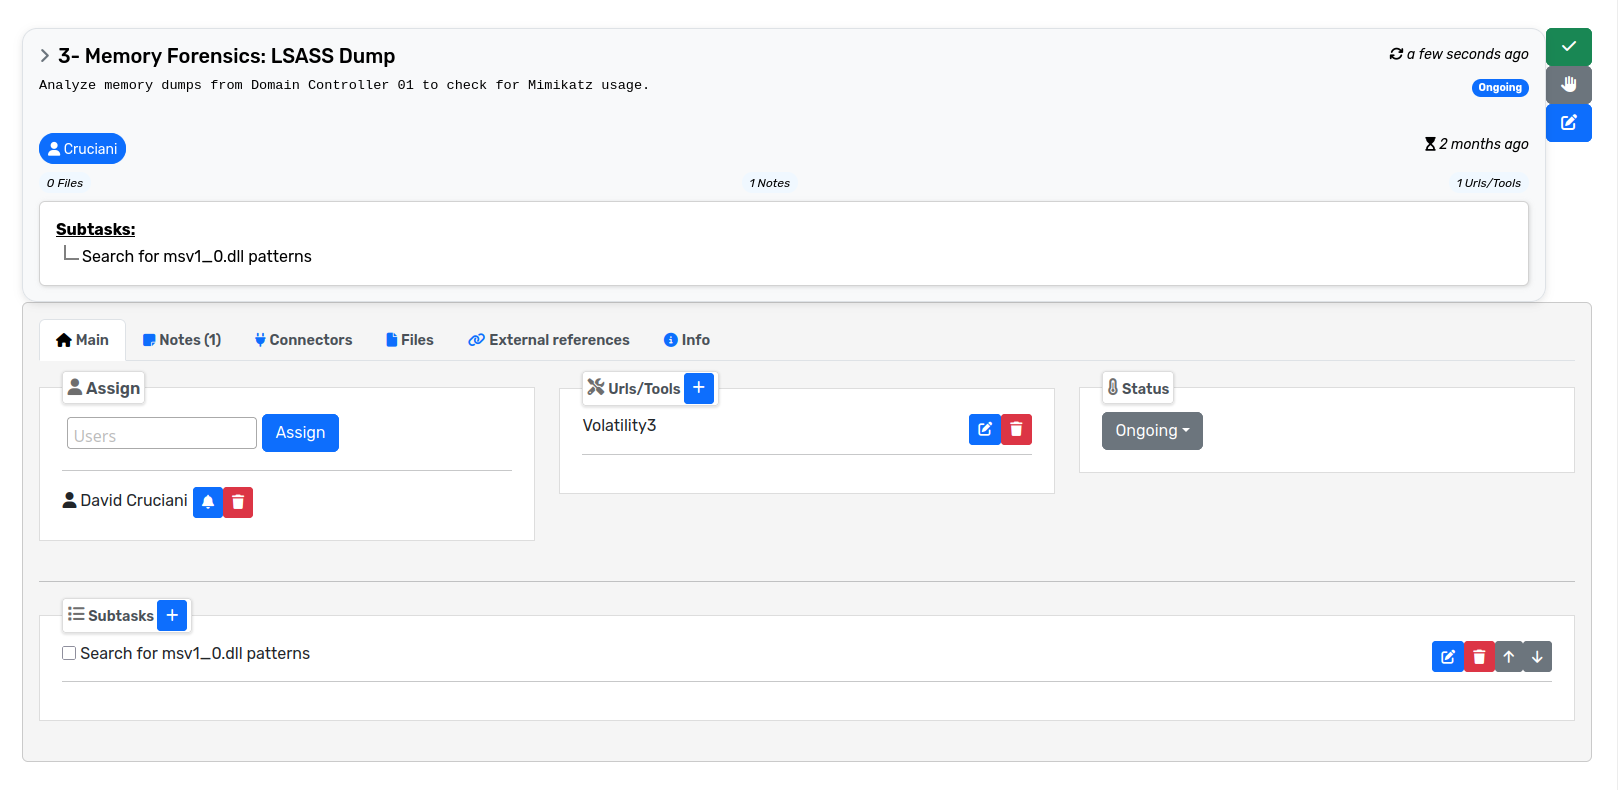
\includegraphics[width=1\textwidth]{img/task_view.png}
	\end{figure}
\end{frame}

\begin{frame}{1. Manage Structured Investigations - templates}
	\begin{figure}[H]
		\centering
		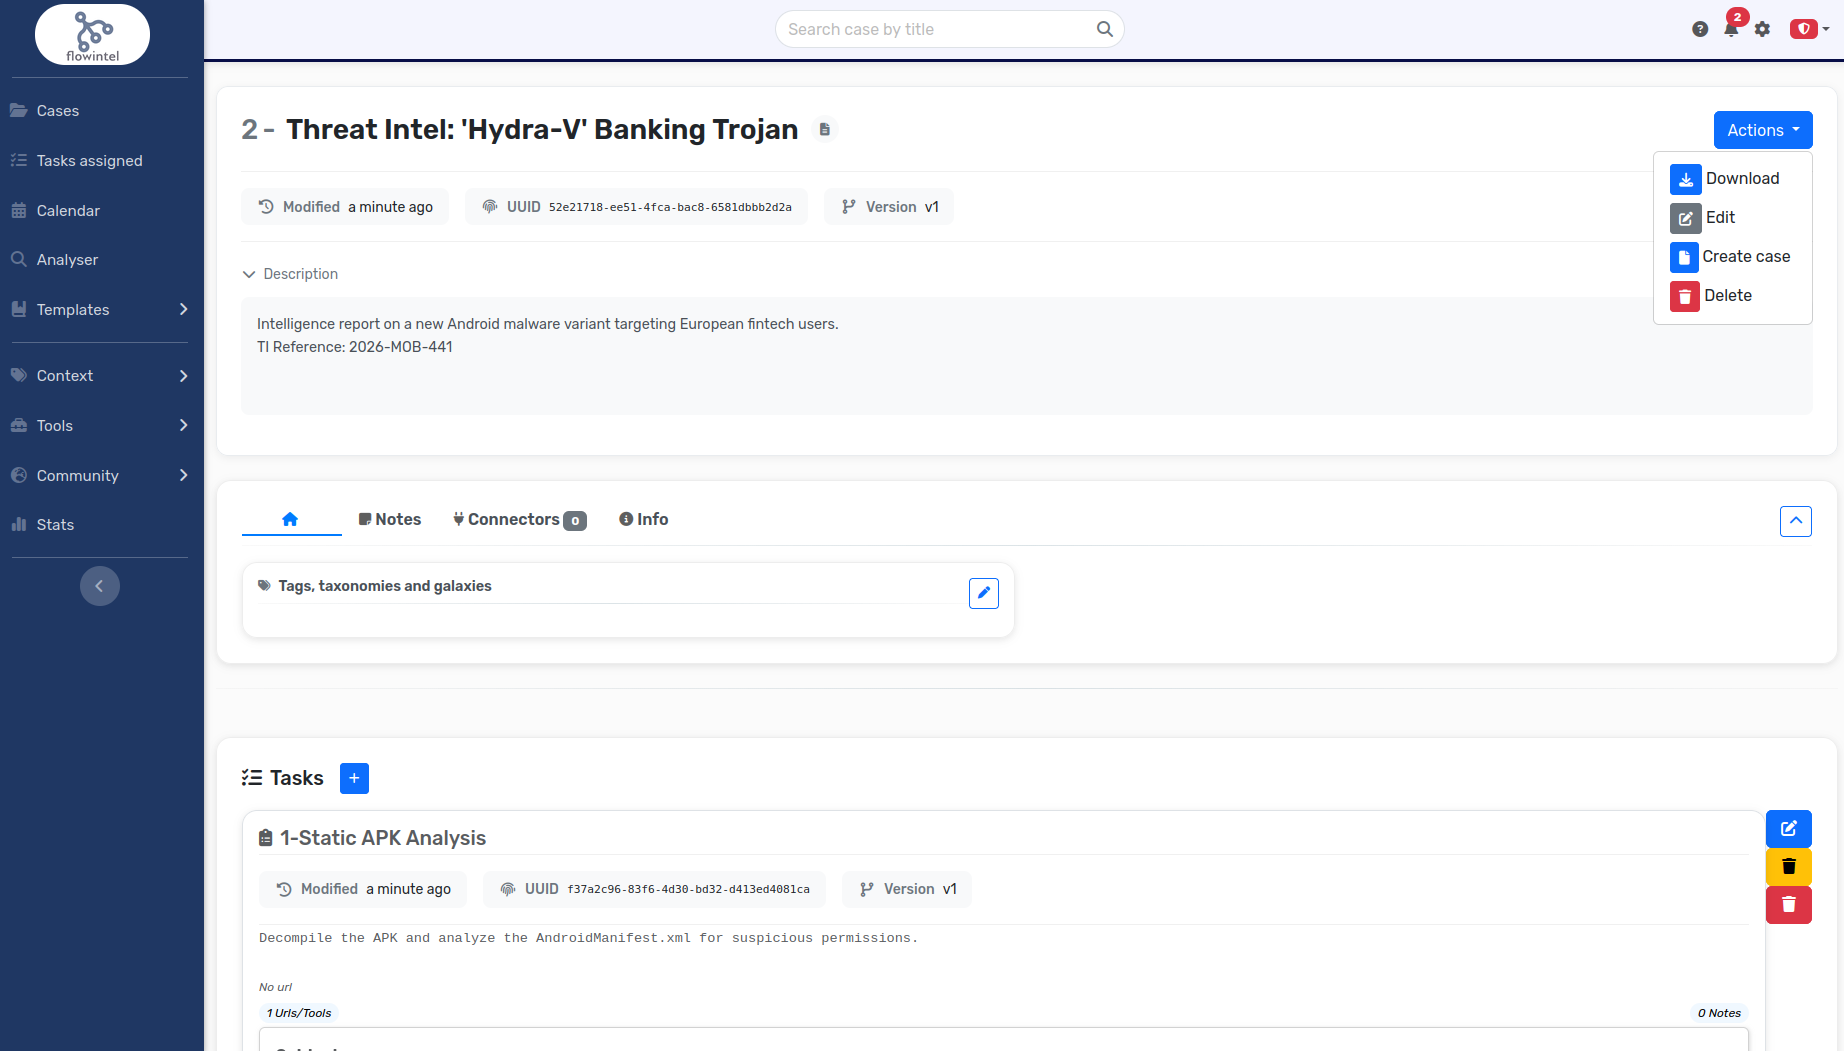
\includegraphics[width=0.95\textwidth]{img/template_view.png}
	\end{figure}
\end{frame}

\begin{frame}{1. Manage Structured Investigations - templates repo}
	\begin{figure}[H]
		\centering
		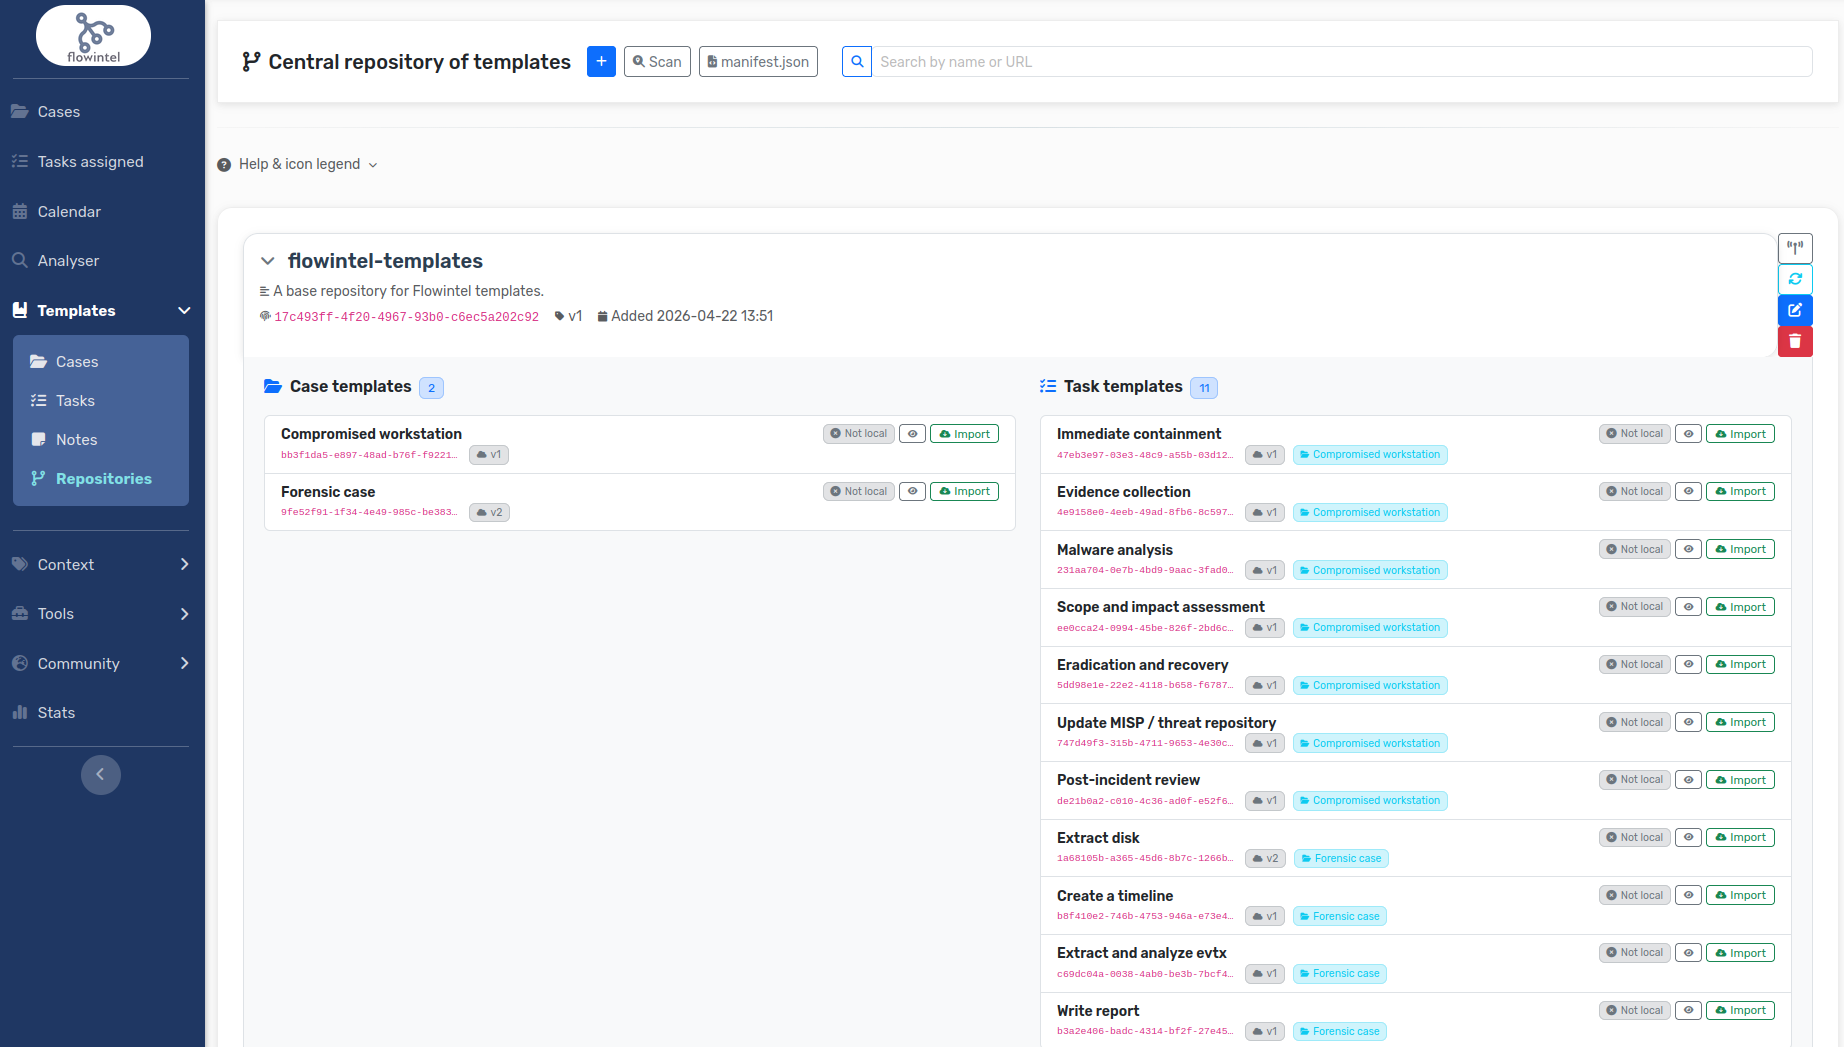
\includegraphics[width=0.95\textwidth]{img/template_repo_view.png}
	\end{figure}
\end{frame}


\section{2. Handle Sensitive \& Privileged Cases}

\begin{frame}{2. Handle Sensitive \& Privileged Cases}
\begin{itemize}
    \item Create privileged cases with restricted access
    \item Assign roles with specific permissions: 
	\begin{itemize}
		\item Case Admin can create cases
		\item Queue Admin can accept tasks
		\item Queuer can create tasks and await approval
	\end{itemize}
    \item Prevent unauthorized deletion, merging, or closure
    \item Enforce organization-level visibility
\end{itemize}
\end{frame}

\begin{frame}{2. Handle Sensitive \& Privileged Cases}
	\begin{figure}[H]
		\centering
		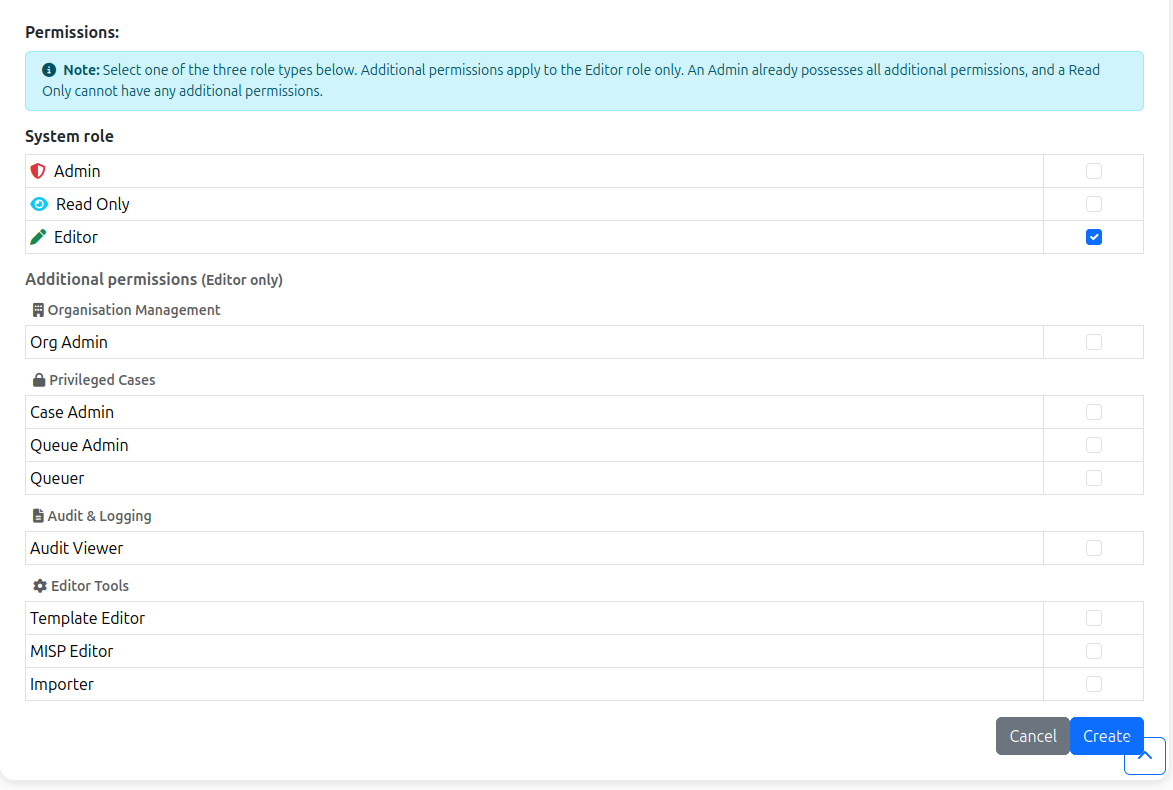
\includegraphics[width=0.8\textwidth]{img/roles.png}
	\end{figure}
\end{frame}

\begin{frame}{2. Handle Sensitive \& Privileged Cases}
	Case View:
	\begin{figure}[H]
		\centering
		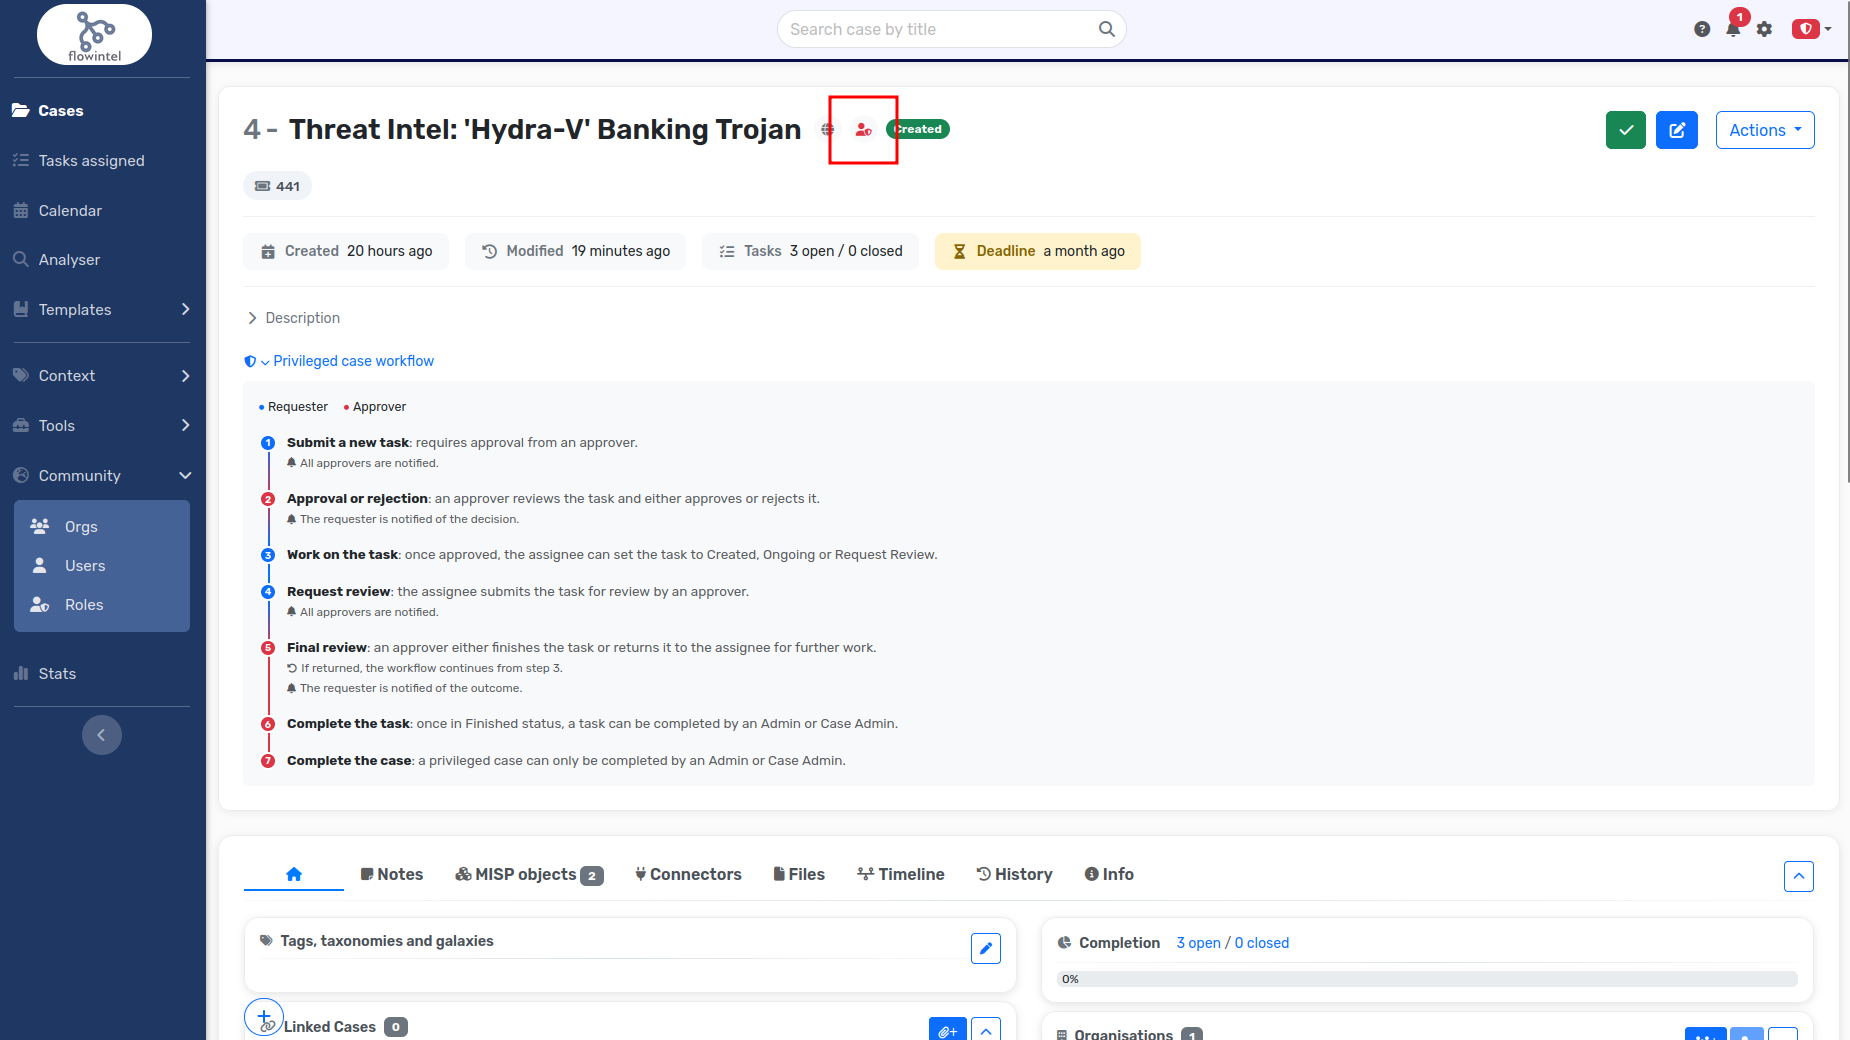
\includegraphics[width=1\textwidth]{img/privilege_case_view.png}
	\end{figure}
\end{frame}

\begin{frame}{2. Handle Sensitive \& Privileged Cases}
	Task view:
	\begin{figure}[H]
		\centering
		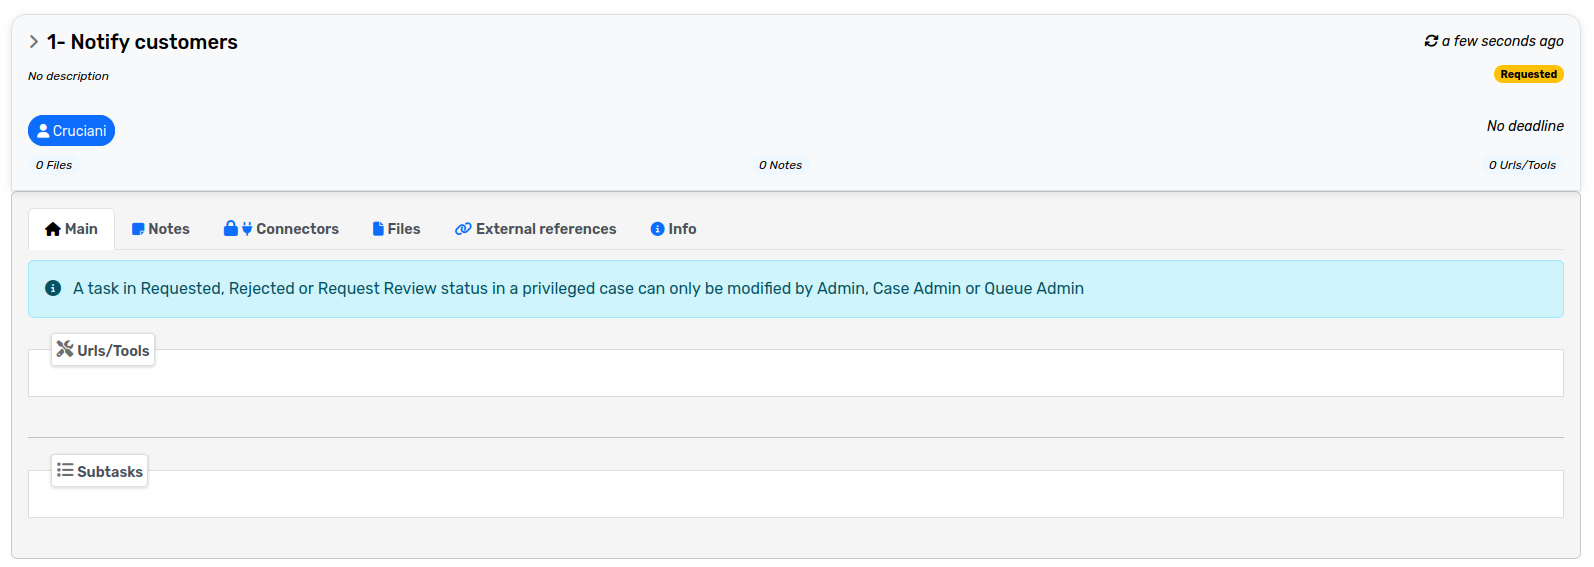
\includegraphics[width=1\textwidth]{img/privilege_task_view.png}
	\end{figure}
\end{frame}

\section{3. Document and Preserve Evidence}

\begin{frame}{3. Document and Preserve Evidence}
\begin{itemize}
    \item Attach files to cases and tasks
    \item Store forensic exports (CSV, JSON, TXT)
    \item Convert imported files into structured notes
    \item Record external references (OSINT, reports, URLs)
    \item Track file metadata (size, type, timestamp)
\end{itemize}
\end{frame}

\begin{frame}{3. Document and Preserve Evidence}
	\begin{figure}[H]
		\centering
		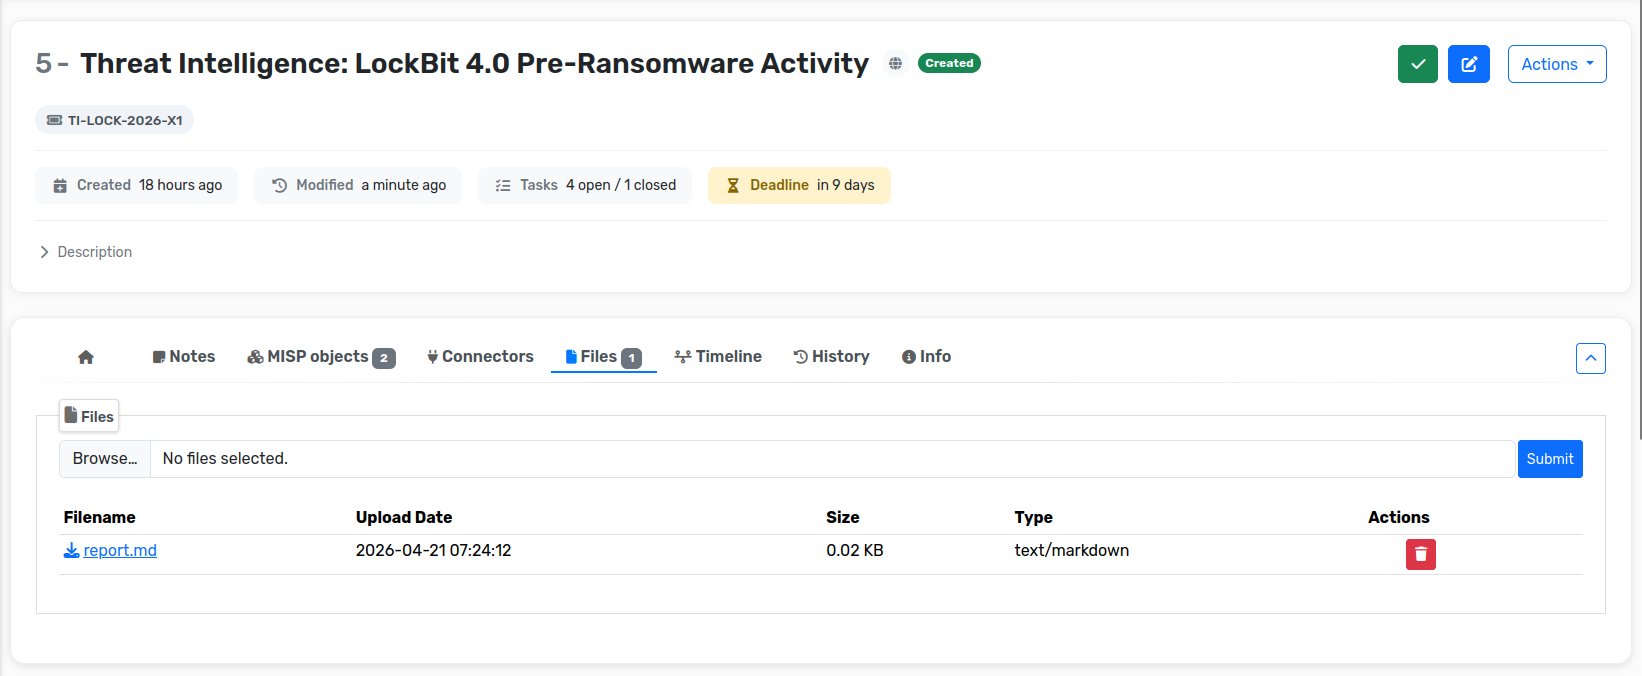
\includegraphics[width=1\textwidth]{img/file_view.png}
	\end{figure}
\end{frame}

\section{4. Maintain Full Audit \& Accountability}

\begin{frame}{4. Maintain Full Audit \& Accountability}
\begin{itemize}
    \item Comprehensive audit trail of actions
    \item Log case creation, edits, deletions
    \item Track task state changes
    \item Record role and permission changes
    \item Dedicated Audit Viewer role
\end{itemize}
\end{frame}

\begin{frame}{4. Maintain Full Audit \& Accountability}
	\begin{figure}[H]
		\centering
		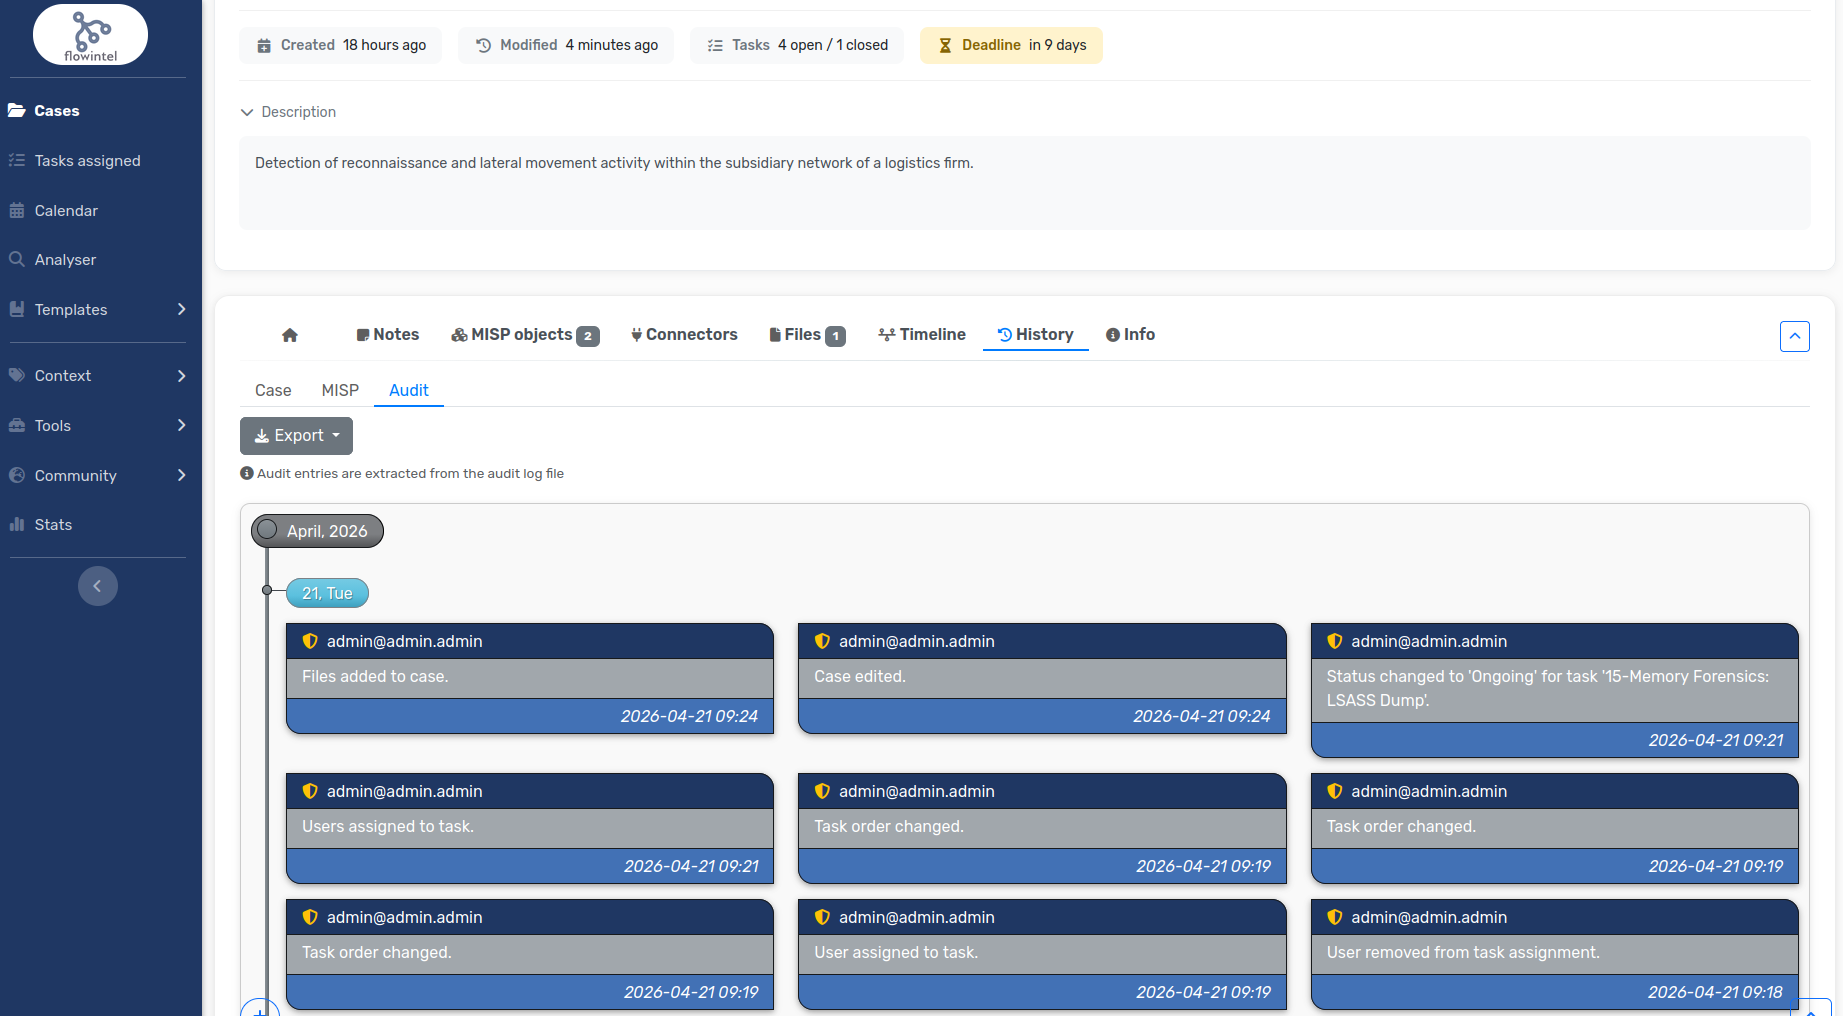
\includegraphics[width=0.9\textwidth]{img/audit_view.png}
	\end{figure}
\end{frame}

\section{5. Multi-Agency \& Organizational Control}

\begin{frame}{5. Multi-Agency \& Organizational Control}
\begin{itemize}
    \item Organization-based visibility restrictions
    \item OrgAdmin role for delegated administration
    \item Prevent deletion of organizations owning cases
    \item Statistics per organization and user
\end{itemize}
\end{frame}

\begin{frame}{5. Multi-Agency \& Organizational Control}
	\begin{figure}[H]
		\centering
		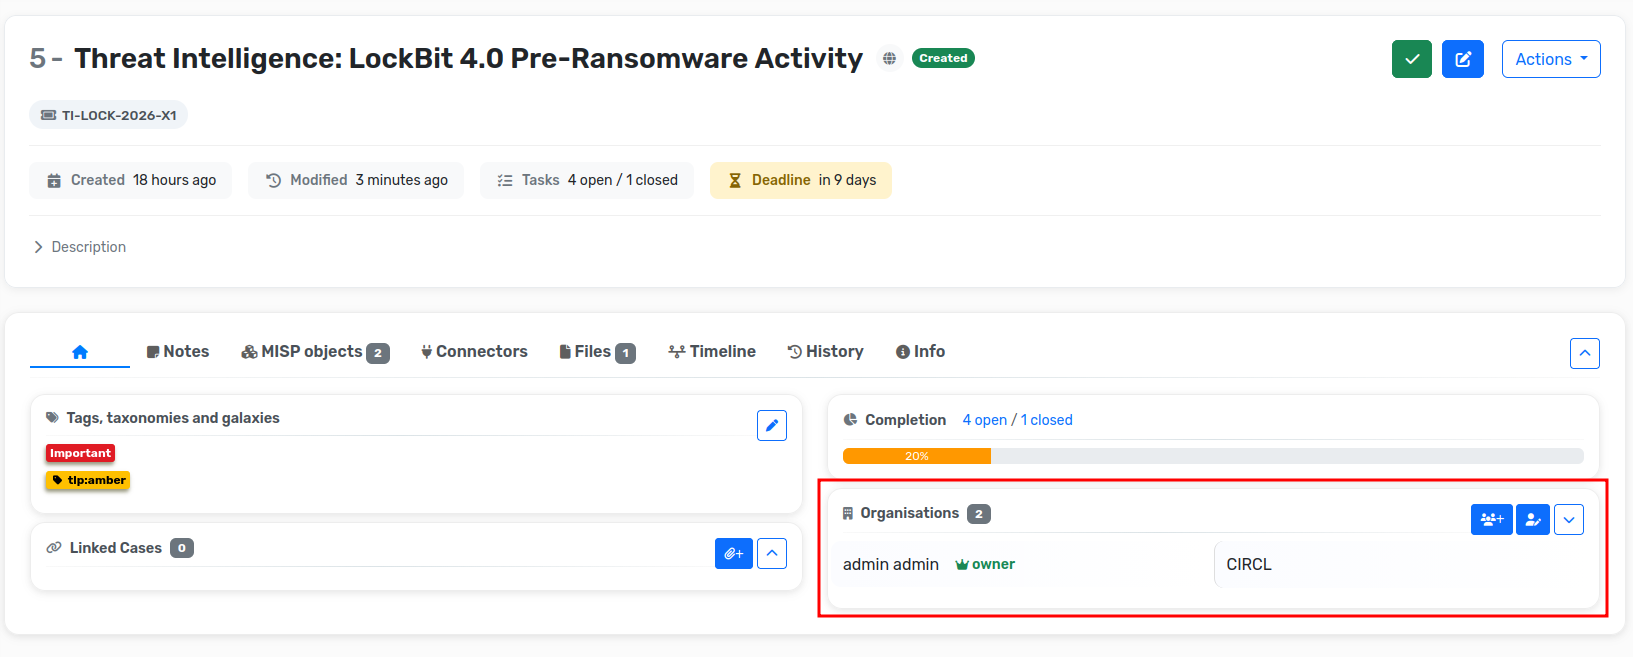
\includegraphics[width=1\textwidth]{img/orgs_in_case.png}
	\end{figure}
\end{frame}

\section{6. Integrate Threat Intelligence (MISP)}

\begin{frame}{6. Integrate Threat Intelligence (MISP)}
\begin{itemize}
    \item Manage MISP objects inside cases
    \item Send case or just objects to MISP
    \item Create a case from a MISP event
    \item Synchronize cases with MISP events
    \item Use taxonomies and galaxies for classification
    \item Import custom taxonomies and galaxies
	\item MISP-modules integration for enrichment and analysis
\end{itemize}
\end{frame}

\begin{frame}{6. Integrate Threat Intelligence (MISP)}
	\begin{figure}[H]
		\centering
		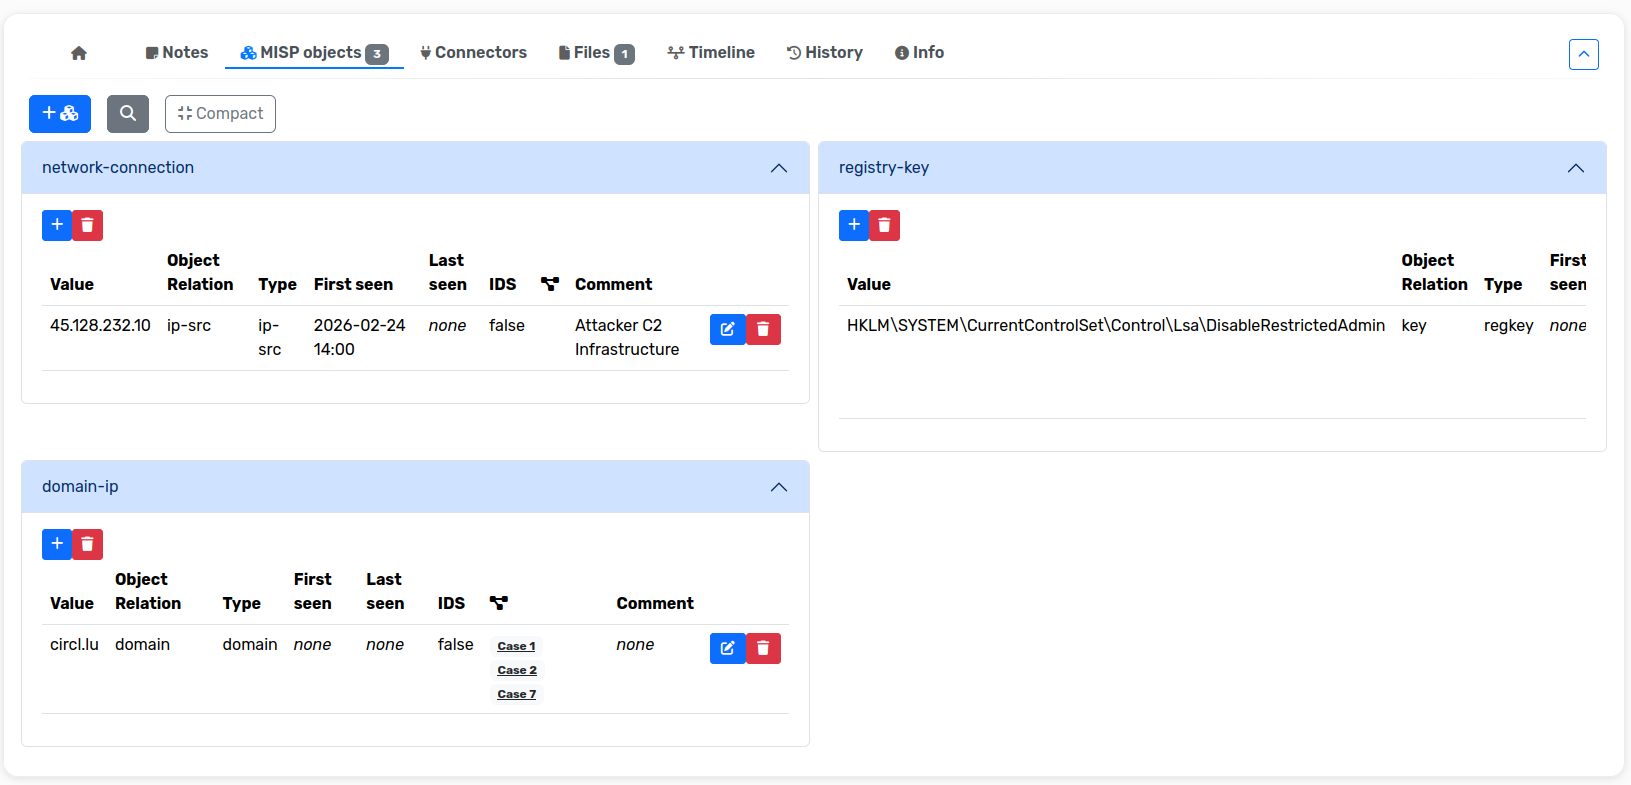
\includegraphics[width=1\textwidth]{img/misp_objects_view.png}
	\end{figure}
\end{frame}

\begin{frame}{6. Integrate Threat Intelligence (MISP)}
	\centering
	\Large
	Quick Demo!\\
	\bigskip
\end{frame}

\section{7. Operational Coordination}

\begin{frame}{7. Operational Coordination}
\begin{itemize}
    \item Task notifications and overdue tracking
    \item Calendar view with ICS export
    \item Full calendar feed API
    \item Progress indicators and workload overview
\end{itemize}
\end{frame}

\begin{frame}{7. Operational Coordination}
	\begin{figure}[H]
		\centering
		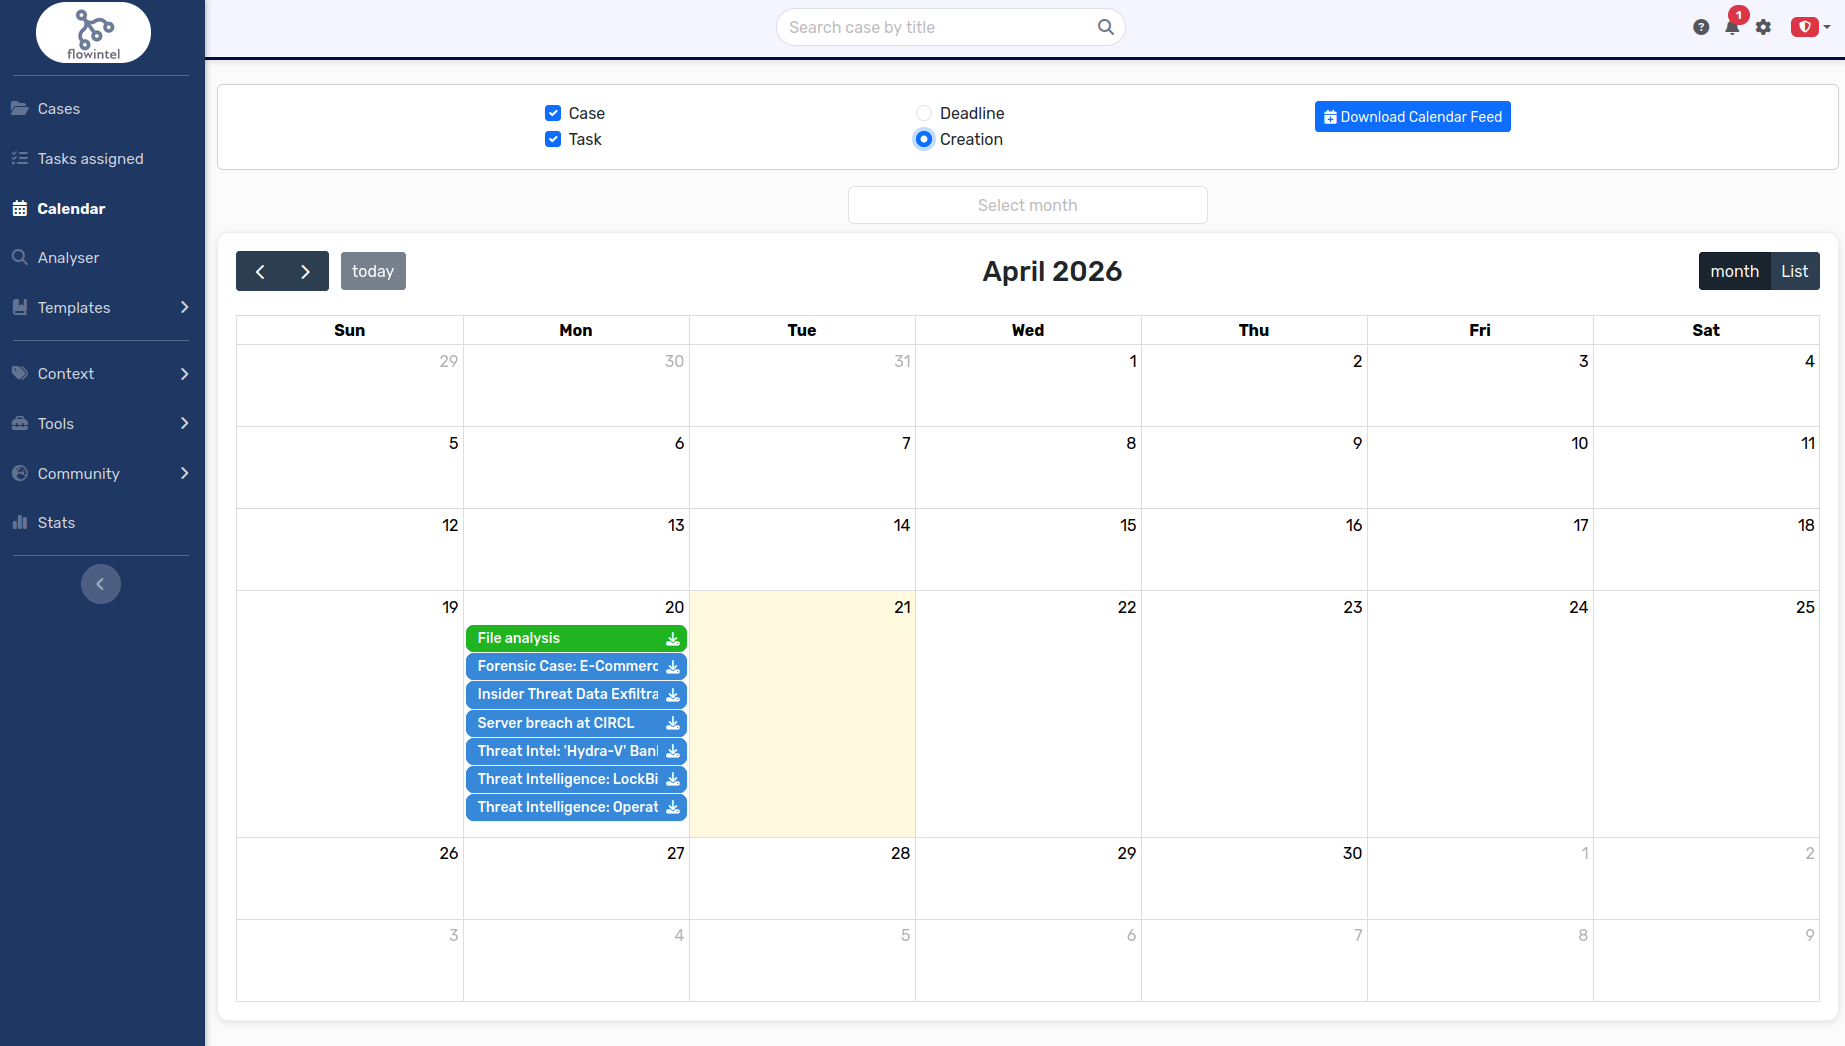
\includegraphics[width=0.9\textwidth]{img/calendar.png}
	\end{figure}
\end{frame}


\section{8. Dashboard}

\begin{frame}{8. Dashboard}
	\begin{figure}[H]
		\centering
		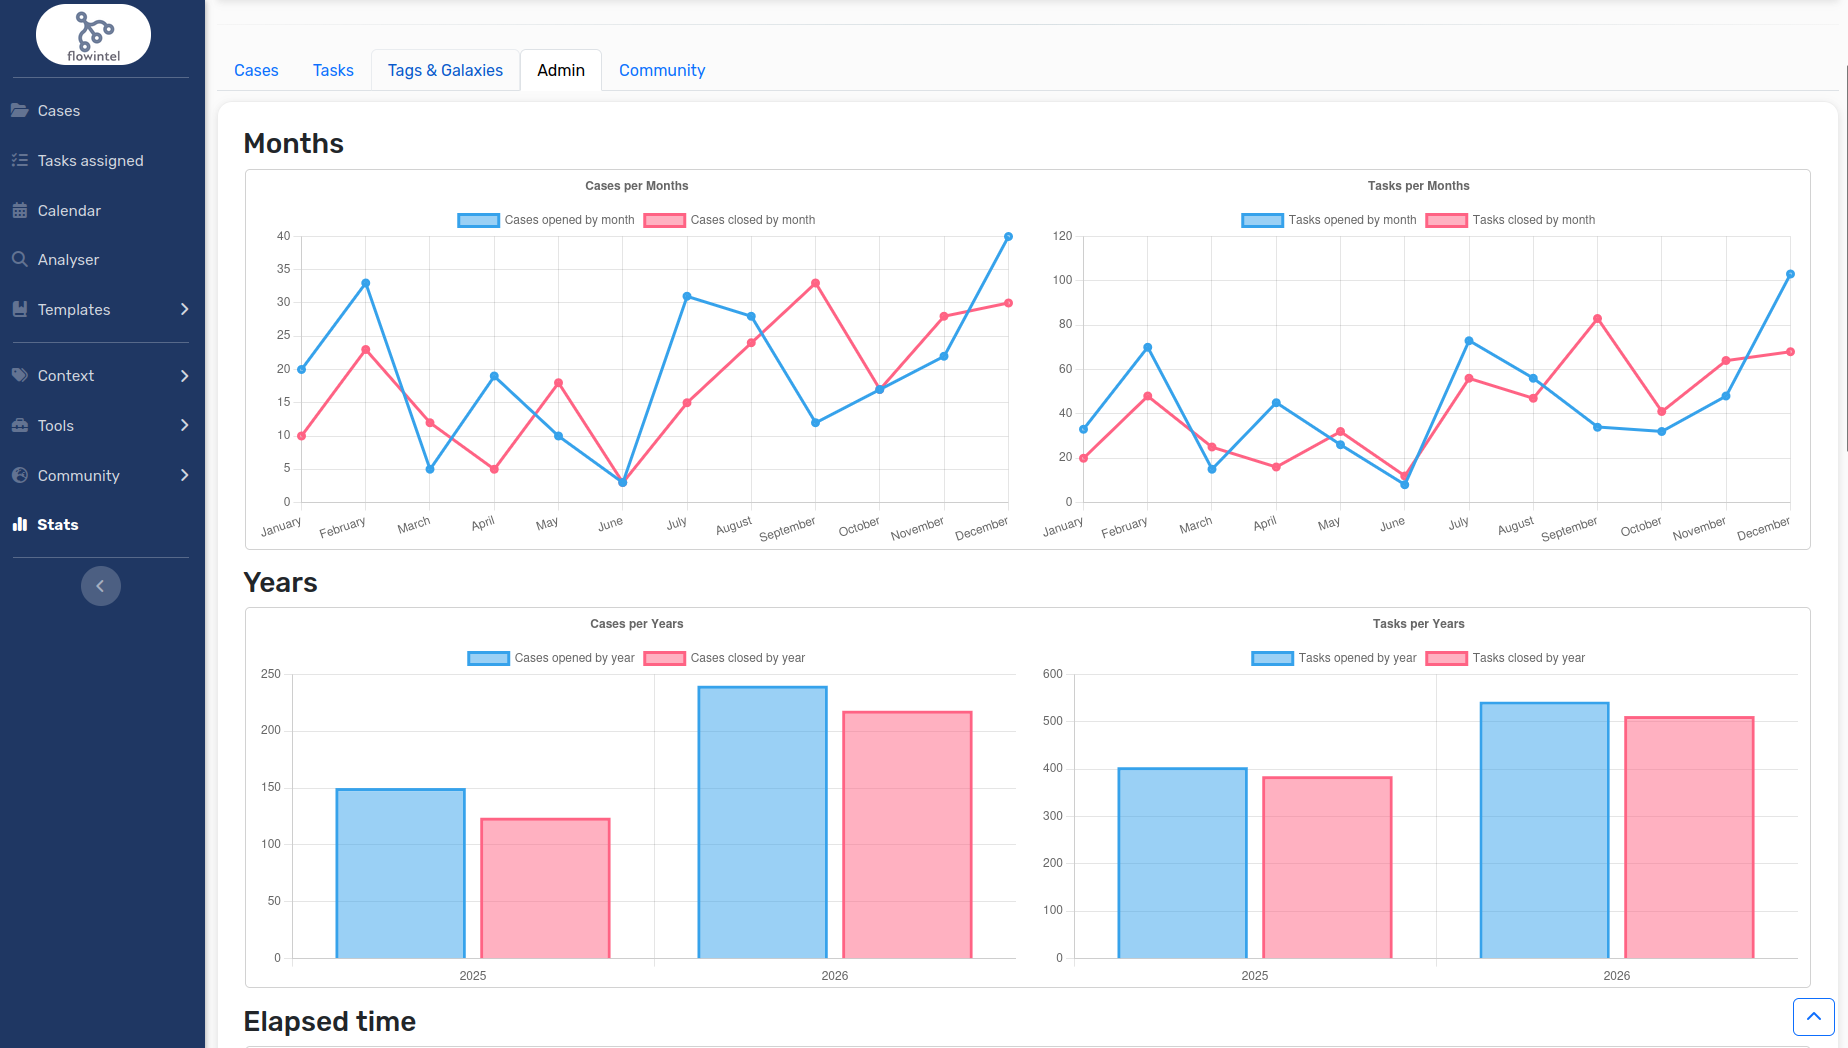
\includegraphics[width=0.9\textwidth]{img/admin_stats.png}
	\end{figure}
\end{frame}

\begin{frame}{8. Dashboard}
	\begin{figure}[H]
		\centering
		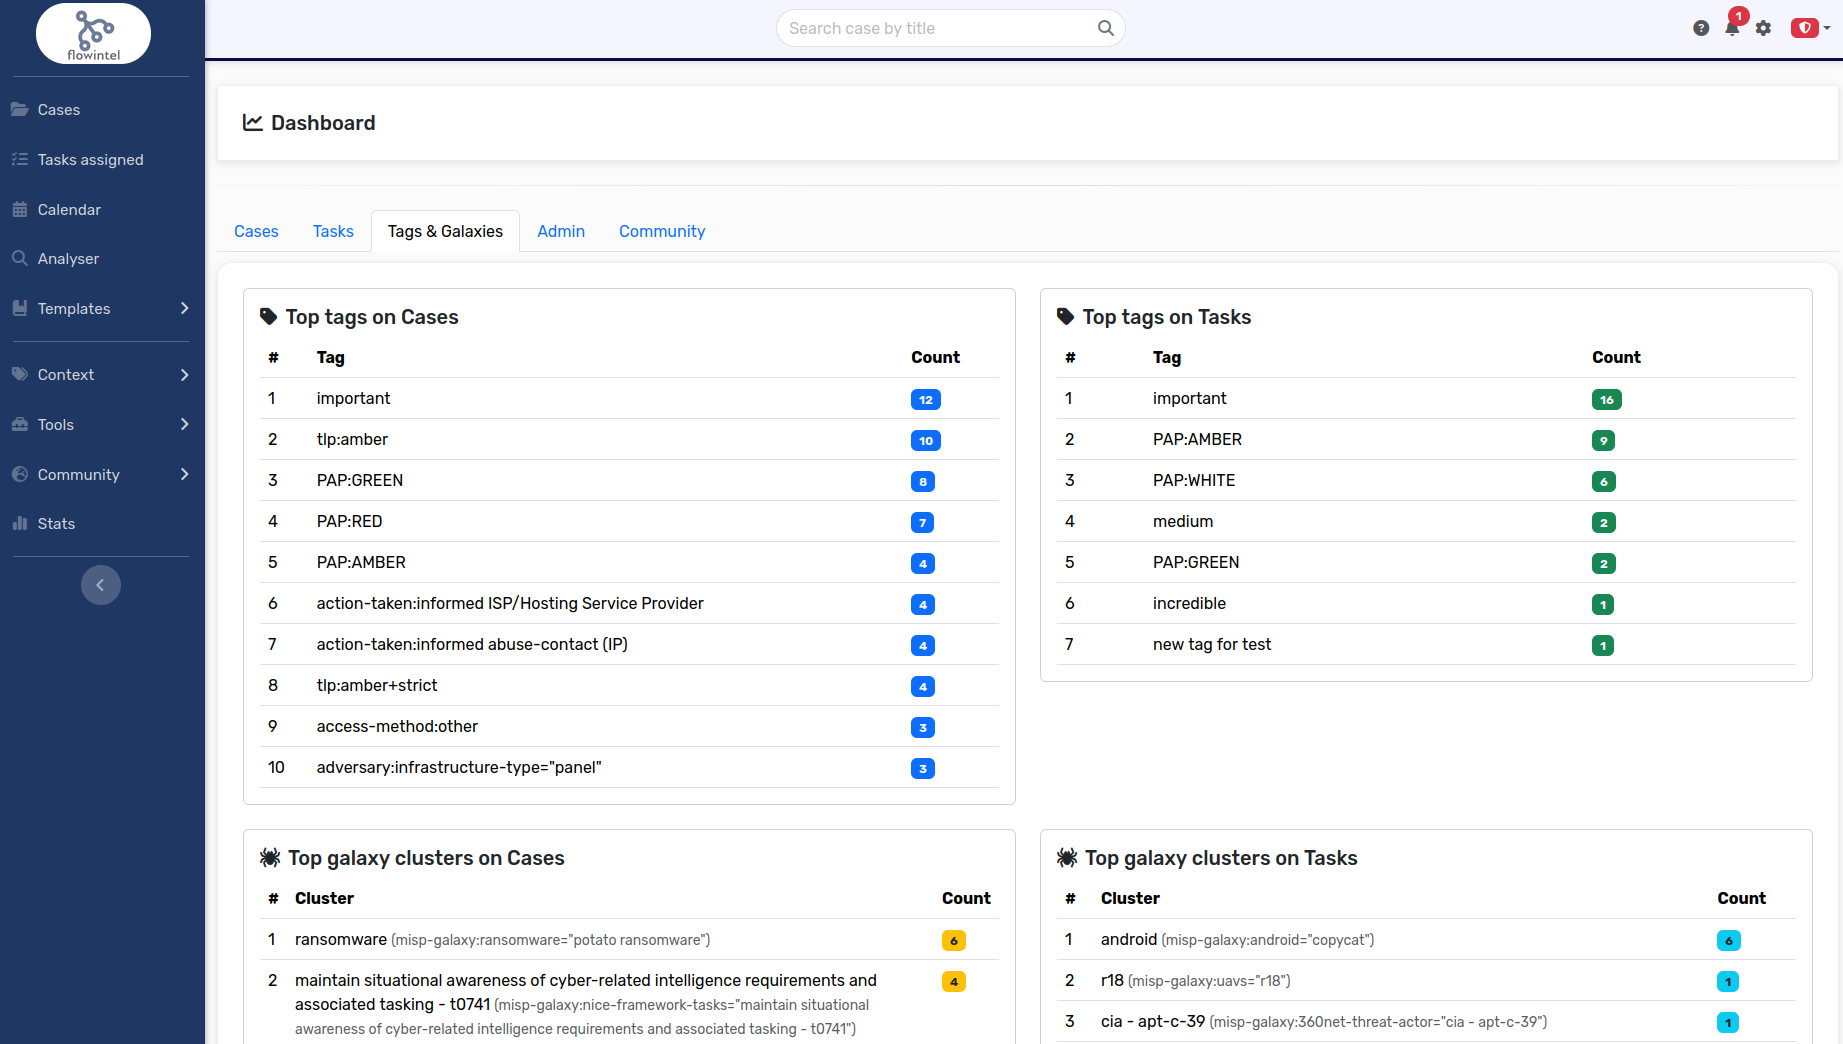
\includegraphics[width=0.9\textwidth]{img/tags_stats.png}
	\end{figure}
\end{frame}

\begin{frame}{Other features present in Flowintel}
	\begin{itemize}
		\item Attribute value search functionality
		\item Importer for cases and templates
		\item Template repository support
		\item Bulk exporter
		\item Flowrefs inside notes
		\item API and Library\footnote{\url{https://github.com/AbstractionsLab/PyFlowintel}}
	\end{itemize}
\end{frame}

\begin{frame}{Strategic Value for LEA}
	\begin{itemize}
		\item Structured investigative workflow
		\item Strong governance and auditability
		\item Secure multi-agency collaboration
		\item Integrated intelligence handling
		\item Open-source and adaptable
	\end{itemize}
\end{frame}

\begin{frame}{The end}
	\centering
	\Large
	Thanks for your attention!\\
	\bigskip
\end{frame}

\end{document}
